%% ============================================================================
%% Kernel-Talk Architecture Document
%% A Digital Twin for the Linux Kernel
%%
%% Compile with:
%%   pdflatex architecture.tex
%%   pdflatex architecture.tex   (twice for cross-references)
%%
%% Requirements: texlive-full or equivalent (TikZ, listings, geometry, etc.)
%% ============================================================================

\documentclass[11pt,a4paper]{article}

%% ── Packages ─────────────────────────────────────────────────────────────────
\usepackage[margin=2.5cm]{geometry}
\usepackage[T1]{fontenc}
\usepackage[utf8]{inputenc}
\usepackage{microtype}
\usepackage{lmodern}
\usepackage{amsmath,amssymb}
\usepackage{graphicx}
\usepackage{xcolor}
\usepackage{hyperref}
\usepackage{booktabs}
\usepackage{longtable}
\usepackage{array}
\usepackage{enumitem}
\usepackage{titlesec}
\usepackage{fancyhdr}
\usepackage{listings}
\usepackage{caption}
\usepackage{subcaption}
\usepackage{float}
\usepackage[most]{tcolorbox}
%\usepackage{fontawesome5}  % optional: install texlive-fonts-extra if desired

%% TikZ and libraries
\usepackage{tikz}
\usetikzlibrary{
  arrows.meta,
  positioning,
  shapes.geometric,
  shapes.multipart,
  fit,
  backgrounds,
  shadows,
  decorations.pathreplacing,
  calc,
  matrix,
  trees
}

%% ── Colour Palette ───────────────────────────────────────────────────────────
\definecolor{layer1}{HTML}{1A6B3C}   % Source   — deep green
\definecolor{layer2}{HTML}{1F5FA6}   % Binary   — steel blue
\definecolor{layer3}{HTML}{7B2D8B}   % Live sym — purple
\definecolor{layer4}{HTML}{C0392B}   % Memory   — red
\definecolor{mirror}{HTML}{2E86AB}   % Mirror   — teal
\definecolor{probe}{HTML}{E07B39}    % Probe    — amber
\definecolor{synth}{HTML}{6B4226}    % Synth    — brown
\definecolor{train}{HTML}{3D5A80}    % Training — navy
\definecolor{codebg}{HTML}{F7F7F7}
\definecolor{accent}{HTML}{E8B86D}
\definecolor{darkgrey}{HTML}{444444}
\definecolor{lightgrey}{HTML}{EEEEEE}
\definecolor{arrowgrey}{HTML}{888888}

%% ── Hyperref setup ───────────────────────────────────────────────────────────
\hypersetup{
  colorlinks=true,
  linkcolor=layer2,
  urlcolor=layer3,
  citecolor=layer1,
  pdftitle={Kernel-Talk Architecture},
  pdfauthor={Lee Ostadi},
}

%% ── Listings (code style) ────────────────────────────────────────────────────
\lstset{
  backgroundcolor=\color{codebg},
  basicstyle=\ttfamily\small,
  breaklines=true,
  frame=single,
  framerule=0.4pt,
  rulecolor=\color{darkgrey!40},
  numbers=left,
  numberstyle=\tiny\color{darkgrey!60},
  numbersep=5pt,
  tabsize=4,
  showstringspaces=false,
  keywordstyle=\color{layer2}\bfseries,
  commentstyle=\color{layer1!70}\itshape,
  stringstyle=\color{layer3},
  language=Python,
}

%% ── Section styling ──────────────────────────────────────────────────────────
\titleformat{\section}{\Large\bfseries\color{darkgrey}}{\thesection}{1em}{}[\titlerule]
\titleformat{\subsection}{\large\bfseries\color{layer2}}{\thesubsection}{1em}{}
\titleformat{\subsubsection}{\normalsize\bfseries\color{layer1!80!black}}{\thesubsubsection}{1em}{}

%% ── Header / Footer ──────────────────────────────────────────────────────────
\pagestyle{fancy}
\fancyhf{}
\fancyhead[L]{\small\textcolor{darkgrey}{\textit{Kernel-Talk Architecture}}}
\fancyhead[R]{\small\textcolor{darkgrey}{\textit{Lee Ostadi --- Digital Twin for Linux}}}
\fancyfoot[C]{\small\thepage}
\renewcommand{\headrulewidth}{0.4pt}

%% ── TikZ node styles ─────────────────────────────────────────────────────────
\tikzset{
  layerbox/.style={
    rectangle, rounded corners=4pt, draw=#1!80!black, fill=#1!12,
    text width=3.8cm, minimum height=1.1cm, align=center,
    font=\small\bfseries, thick
  },
  widelay/.style={
    rectangle, rounded corners=4pt, draw=#1!80!black, fill=#1!12,
    text width=8cm, minimum height=0.95cm, align=left,
    font=\small, thick, inner sep=6pt
  },
  modbox/.style={
    rectangle, rounded corners=3pt, draw=darkgrey!60, fill=white,
    text width=3.2cm, minimum height=0.85cm, align=center,
    font=\footnotesize
  },
  databox/.style={
    rectangle, draw=accent!80, fill=accent!15,
    text width=2.5cm, minimum height=0.7cm, align=center,
    font=\footnotesize\ttfamily, rounded corners=2pt
  },
  arrowstyle/.style={
    -Stealth, thick, color=arrowgrey
  },
  colorarrow/.style={
    -Stealth, very thick, color=#1
  },
  annot/.style={
    font=\scriptsize\itshape, color=darkgrey!70
  },
}

%% ── Utility commands ─────────────────────────────────────────────────────────
\newcommand{\coderef}[1]{\texttt{\small\color{layer2}#1}}
\newcommand{\layerbadge}[2]{%
  \tikz[baseline=(n.base)]\node[
    fill=#1!20, draw=#1!60, rounded corners=2pt,
    inner sep=2pt, font=\scriptsize\bfseries, text=#1!80!black
  ](n){#2};%
}

%% ============================================================================
\begin{document}

%% ── Title Page ───────────────────────────────────────────────────────────────
\begin{titlepage}
\centering
\vspace*{2cm}

{\Huge\bfseries\color{darkgrey} Kernel-Talk}\\[0.3cm]
{\Large\color{layer2} A Digital Twin for the Linux Kernel}\\[0.2cm]
{\normalsize\color{darkgrey!70}\itshape Architecture \& System Design Reference}

\vspace{1.5cm}

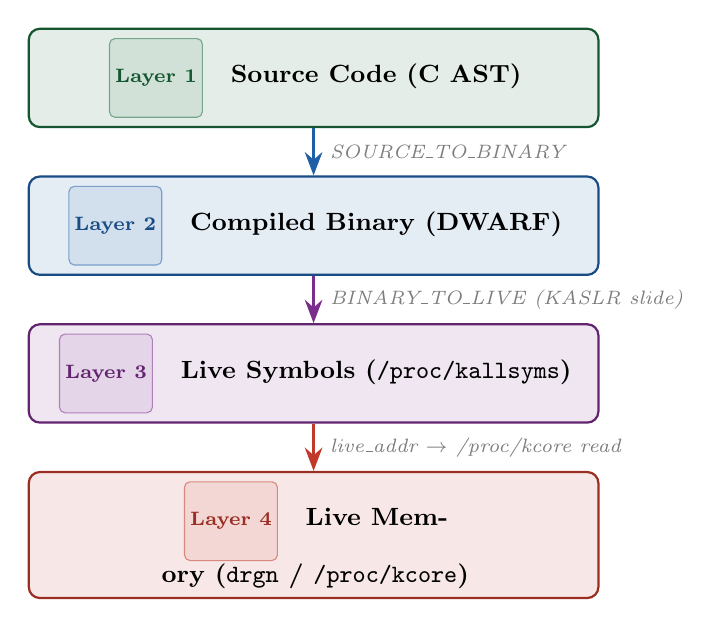
\begin{tikzpicture}[node distance=0.6cm]
  \node[layerbox=layer1, text width=7cm, minimum height=1.0cm]
    (l1) {\layerbadge{layer1}{Layer 1} \; Source Code (C AST)};
  \node[layerbox=layer2, text width=7cm, minimum height=1.0cm, below=of l1]
    (l2) {\layerbadge{layer2}{Layer 2} \; Compiled Binary (DWARF)};
  \node[layerbox=layer3, text width=7cm, minimum height=1.0cm, below=of l2]
    (l3) {\layerbadge{layer3}{Layer 3} \; Live Symbols (\texttt{/proc/kallsyms})};
  \node[layerbox=layer4, text width=7cm, minimum height=1.0cm, below=of l3]
    (l4) {\layerbadge{layer4}{Layer 4} \; Live Memory (\texttt{drgn} / \texttt{/proc/kcore})};

  \draw[colorarrow=layer2] (l1.south) -- (l2.north)
    node[midway,right=2pt,annot]{SOURCE\_TO\_BINARY};
  \draw[colorarrow=layer3] (l2.south) -- (l3.north)
    node[midway,right=2pt,annot]{BINARY\_TO\_LIVE (KASLR slide)};
  \draw[colorarrow=layer4] (l3.south) -- (l4.north)
    node[midway,right=2pt,annot]{live\_addr $\to$ /proc/kcore read};
\end{tikzpicture}

\vspace{1.5cm}

\begin{tcolorbox}[
  colback=codebg, colframe=darkgrey!40,
  width=10cm, arc=4pt, boxrule=0.6pt
]
\small\centering
\textit{``Vector search tells you what code looks like what you asked about.\\
Graph traversal tells you what it depends on.\\
drgn tells you what is actually happening right now.''}
\end{tcolorbox}

\vfill
{\large Lee Ostadi}\\[0.2cm]
{\normalsize\color{darkgrey!70} Graduate Researcher --- Machine Learning \& Neural Networks}\\[0.1cm]
{\small\color{darkgrey!60} \today}
\end{titlepage}

%% ── Table of Contents ────────────────────────────────────────────────────────
\tableofcontents
\newpage

%% ============================================================================
\section{System Overview}
\label{sec:overview}
%% ============================================================================

Kernel-Talk is a \textbf{Digital Twin} for the Linux kernel: a system that
simultaneously holds the static source structure of the kernel (its theory)
and its live runtime state (its reality), fusing them through language models
to answer questions that neither source code search nor runtime debugging can
answer alone.

The central claim is that understanding why a kernel behaviour occurs requires
traversing \emph{four distinct representations} of the same artefact:

\begin{enumerate}[leftmargin=2em, itemsep=2pt]
  \item \textbf{C source code} --- the human-readable expression of intent,
        parsed into a semantic graph by tree-sitter.
  \item \textbf{Compiled binary} (vmlinux DWARF) --- the compiled truth:
        function address ranges, struct field byte offsets, inlining decisions.
  \item \textbf{Live symbol table} (\texttt{/proc/kallsyms}) --- the
        KASLR-adjusted addresses of every exported kernel symbol \emph{in the
        running kernel}.
  \item \textbf{Live memory} (drgn / \texttt{/proc/kcore}) --- actual struct
        field values at runtime, without stopping execution.
\end{enumerate}

These are not independent datastores. They are connected by precise
mathematical relationships (KASLR slide, DWARF offset tables) encoded as
typed edges in a unified \textbf{KernelGraph}. The architecture is designed
so that any question can be traced from a user's natural-language query
through all four layers to a grounded, citable answer.

%% ── Query pipeline narrative ─────────────────────────────────────────────────
\subsection{End-to-End Query Path}

\begin{center}
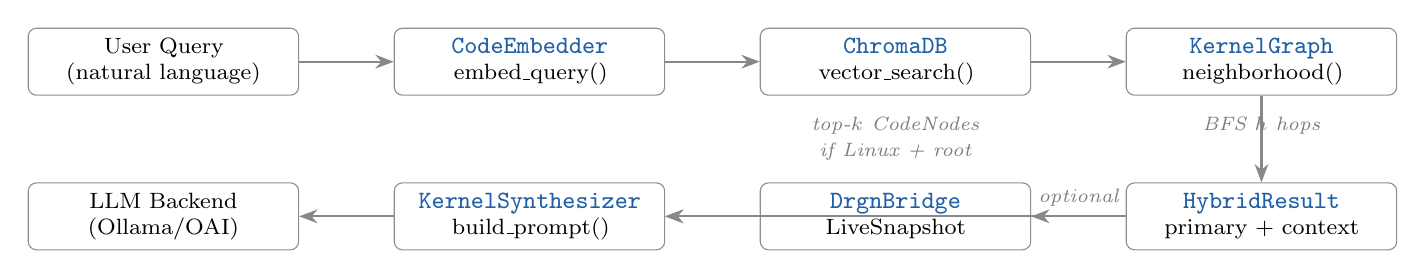
\begin{tikzpicture}[node distance=0.45cm and 0.5cm, every node/.style={font=\small}]

  \node[modbox] (q) {User Query\\(natural language)};
  \node[modbox, right=1.2cm of q] (emb) {\coderef{CodeEmbedder}\\embed\_query()};
  \node[modbox, right=1.2cm of emb] (vec) {\coderef{ChromaDB}\\vector\_search()};
  \node[modbox, right=1.2cm of vec] (gph) {\coderef{KernelGraph}\\neighborhood()};

  \node[modbox, below=1.1cm of gph] (hr) {\coderef{HybridResult}\\primary + context};
  \node[modbox, left=1.2cm of hr]   (drgn) {\coderef{DrgnBridge}\\LiveSnapshot};
  \node[modbox, left=1.2cm of drgn] (synth) {\coderef{KernelSynthesizer}\\build\_prompt()};
  \node[modbox, left=1.2cm of synth] (llm) {LLM Backend\\(Ollama/OAI)};

  \draw[arrowstyle] (q)   -- (emb);
  \draw[arrowstyle] (emb) -- (vec);
  \draw[arrowstyle] (vec) -- (gph);
  \draw[arrowstyle] (gph) -- (hr);
  \draw[arrowstyle] (hr)  -- (drgn)
    node[midway,above,annot]{optional};
  \draw[arrowstyle] (drgn) -- (synth);
  \draw[arrowstyle] (hr)   -- (synth);
  \draw[arrowstyle] (synth) -- (llm);

  \node[annot, below=0.15cm of vec] {top-$k$ CodeNodes};
  \node[annot, below=0.15cm of gph] {BFS $h$ hops};
  \node[annot, above=0.15cm of drgn] {if Linux + root};
\end{tikzpicture}
\end{center}

\noindent
The query pipeline is a two-stage retrieval followed by generative synthesis.
Stage 1 (\emph{retrieve}) is entirely offline-capable---it uses pre-built
vector and graph indices. Stage 2 (\emph{synthesize}) calls an LLM with a
structured prompt containing the retrieved code context and optional live
state. The LLM backend is pluggable: Ollama (default, offline),
OpenAI-compatible, or Anthropic.

%% ============================================================================
\section{Repository Structure}
\label{sec:structure}
%% ============================================================================

\begin{tcolorbox}[
  colback=codebg, colframe=darkgrey!30, arc=4pt,
  title={\small\ttfamily kernel-talk/ --- top-level layout},
  fonttitle=\bfseries\small
]
\begin{lstlisting}[language={}, numbers=none, frame=none,
                   backgroundcolor=\color{codebg}, basicstyle=\ttfamily\small]
kernel-talk/
|-- cli/
|   `-- ktalk.py              # CLI entry point (argparse commands)
|-- core/
|   |-- mirror/               # The Mirror: static code twin
|   |   |-- parser.py         # KernelParser, CodeNode, tree-sitter queries
|   |   |-- graph.py          # KernelGraph, EdgeType, GraphContext
|   |   |-- embedder.py       # CodeEmbedder (CodeBERT), chunk_text
|   |   `-- store.py          # KernelStore: unified retrieval interface
|   |-- dwarf/
|   |   `-- bridge.py         # DwarfBridge, BinarySymbol, StructLayout
|   |-- probe/
|   |   |-- kallsyms.py       # KallsymsBridge, KallsymsEntry, KASLR slide
|   |   `-- drgn_bridge.py    # DrgnBridge, LiveSnapshot, ProcessSnapshot
|   `-- synthesis/
|       `-- synthesizer.py    # KernelSynthesizer, build_prompt
|-- training/
|   |-- mine.py               # TripletMiner: git history -> JSONL
|   |-- bm25.py               # BM25Index: hard negative enrichment
|   |-- dataset.py            # TripletDataset: curriculum-aware DataLoader
|   `-- train_biencoder.py    # BiEncoder fine-tuning with InfoNCE
|-- tools/
|   `-- xray.py               # Filesystem X-Ray (/sys, /proc resolution)
`-- tests/
    |-- test_graph.py         # KernelGraph unit tests
    |-- test_persistence.py   # Save/load roundtrip tests
    |-- test_store.py         # KernelStore integration tests
    `-- test_training.py      # 50 tests: BM25, mining, curriculum
\end{lstlisting}
\end{tcolorbox}

%% ============================================================================
\section{The Mirror --- Static Code Twin}
\label{sec:mirror}
%% ============================================================================

The Mirror is Layer 1 of the Digital Twin. It ingests the entire Linux kernel
C source tree and produces two complementary indices: a \textbf{vector index}
(ChromaDB) for semantic similarity search, and a \textbf{knowledge graph}
(NetworkX MultiDiGraph) for structural context expansion. Both are built from
the same atomic unit: the \coderef{CodeNode}.

%% ── 3.1 CodeNode ─────────────────────────────────────────────────────────────
\subsection{The \texttt{CodeNode} --- Atomic Unit}
\label{sec:codenode}

\begin{tcolorbox}[
  colback=layer1!5, colframe=layer1!50, arc=4pt,
  title={\small\ttfamily core/mirror/parser.py --- CodeNode},
  fonttitle=\bfseries\small\color{layer1!80!black}
]
\begin{lstlisting}
@dataclass
class CodeNode:
    id: str            # "kernel/sched/fair.c::tg_throttle_up"
    node_type: str     # function | struct | union | enum | macro | file
    symbol_name: str   # bare C identifier
    file_path: str     # relative to kernel root
    line_start: int    # 1-indexed
    line_end: int
    code: str          # raw C source text
    docstring: str     # preceding /** ... */ block comment
    calls: list[str]   # callee names (-> CALLS graph edges)
    uses_structs: list[str]  # struct/union refs (-> USES_STRUCT edges)
    includes: list[str]     # #include paths (file nodes only)
\end{lstlisting}
\end{tcolorbox}

A \coderef{CodeNode} is simultaneously:
\begin{itemize}[itemsep=1pt]
  \item A \textbf{graph node} --- its \texttt{id} is the vertex key in \coderef{KernelGraph}.
  \item A \textbf{vector document} --- its \texttt{embedding\_text()} is stored in ChromaDB.
  \item A \textbf{training unit} --- it is the target of BM25 and bi-encoder retrieval.
\end{itemize}

The \coderef{embedding\_text()} method concatenates
\texttt{docstring + ``//~type:~name~in~path'' + code}. The docstring prepend
is critical: kernel developers write highly information-dense block comments
that capture \emph{intent}, while the code body captures \emph{mechanism}.
Fusing both gives the CodeBERT embedding far richer semantic signal than code
alone.

%% ── 3.2 KernelParser ─────────────────────────────────────────────────────────
\subsection{\texttt{KernelParser} --- AST Extraction}
\label{sec:parser}

\coderef{KernelParser} (\texttt{core/mirror/parser.py}) walks the kernel
source tree and extracts \coderef{CodeNode} objects via tree-sitter C queries.
It extracts six node types, each with a dedicated S-expression query:

\begin{center}
\begin{tabular}{@{}llll@{}}
\toprule
\textbf{Node type} & \textbf{tree-sitter tag} & \textbf{Graph edges populated} & \textbf{Notes} \\
\midrule
\texttt{function} & \texttt{function\_definition} & \texttt{CALLS, USES\_STRUCT, DEFINED\_IN} & Primary retrieval target \\
\texttt{struct}   & \texttt{struct\_specifier}    & \texttt{DEFINED\_IN}                      & Layout decoded by DWARF \\
\texttt{union}    & \texttt{union\_specifier}     & \texttt{DEFINED\_IN}                      & Anonymous unions flattened (F-16) \\
\texttt{enum}     & \texttt{enum\_specifier}      & \texttt{DEFINED\_IN}                      & Constants \\
\texttt{macro}    & \texttt{preproc\_def}         & \texttt{DEFINED\_IN}                      & Non-trivial values only \\
\texttt{file}     & (synthetic)                   & \texttt{INCLUDES}                         & Header dependency graph \\
\bottomrule
\end{tabular}
\end{center}

\noindent
\textbf{Key design decisions:}
\begin{itemize}[itemsep=2pt]
  \item \textbf{CORE\_STRUCTS} is a \texttt{frozenset} (immutable, thread-safe).
        Every parsed struct/union name is registered into this set dynamically
        to enable \texttt{USES\_STRUCT} edge detection in later files.
  \item \textbf{SKIP\_PATTERNS} filters generated files (\texttt{.mod.c},
        \texttt{.tmp.}), test fixtures, and tools --- noise that degrades embedding
        quality.
  \item \textbf{Size cap:} files exceeding 2 MB are skipped. These are typically
        generated tables (ID tables, firmware blobs) not useful for retrieval.
\end{itemize}

%% ── 3.3 KernelGraph ──────────────────────────────────────────────────────────
\subsection{\texttt{KernelGraph} --- Structural Knowledge Graph}
\label{sec:graph}

\coderef{KernelGraph} (\texttt{core/mirror/graph.py}) is a
\texttt{nx.MultiDiGraph} --- directed, with multiple edge types allowed between
the same pair of nodes. It serves as the structural backbone of the entire
Digital Twin.

\subsubsection{Edge Types and Layer Crossings}

\begin{center}
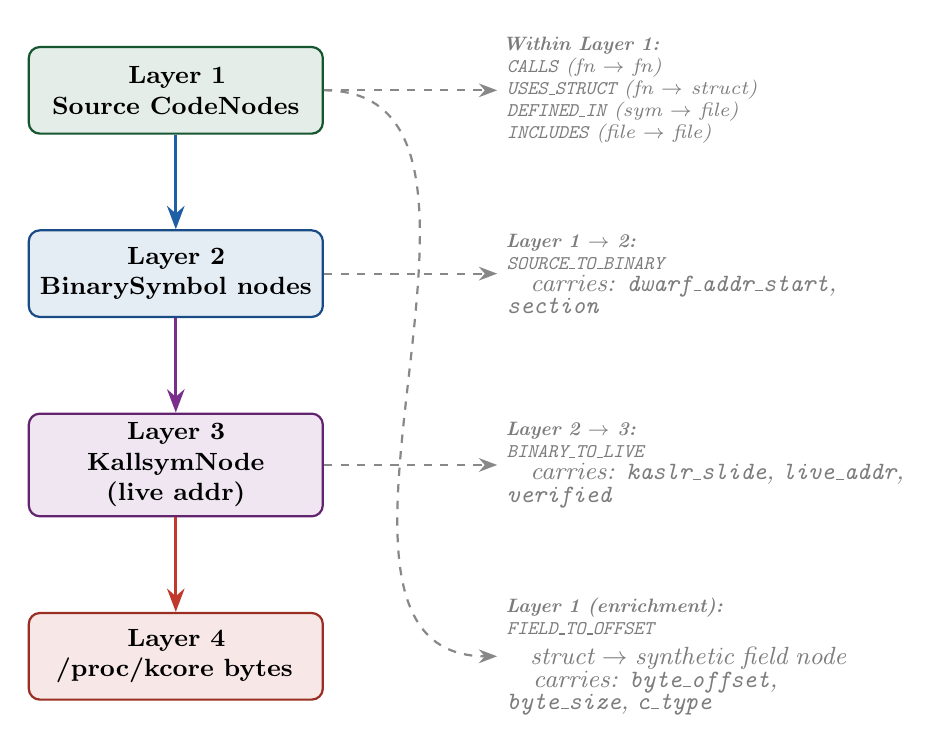
\begin{tikzpicture}[node distance=1.0cm]

  %% Layer boxes (left column)
  \node[layerbox=layer1, text width=3.5cm] (src) {Layer 1\\Source CodeNodes};
  \node[layerbox=layer2, text width=3.5cm, below=1.2cm of src] (bin) {Layer 2\\BinarySymbol nodes};
  \node[layerbox=layer3, text width=3.5cm, below=1.2cm of bin] (kal) {Layer 3\\KallsymNode (live addr)};
  \node[layerbox=layer4, text width=3.5cm, below=1.2cm of kal] (mem) {Layer 4\\/proc/kcore bytes};

  %% Edge annotations (right)
  \node[right=2.2cm of src,  annot, text width=5cm] (e1) {
    \textbf{Within Layer 1:}\\
    \texttt{CALLS} (fn $\to$ fn)\\
    \texttt{USES\_STRUCT} (fn $\to$ struct)\\
    \texttt{DEFINED\_IN} (sym $\to$ file)\\
    \texttt{INCLUDES} (file $\to$ file)
  };
  \node[right=2.2cm of bin,  annot, text width=5cm] (e2) {
    \textbf{Layer 1 $\to$ 2:}\\
    \texttt{SOURCE\_TO\_BINARY}\\
    \quad\small carries: \texttt{dwarf\_addr\_start}, \texttt{section}
  };
  \node[right=2.2cm of kal,  annot, text width=5cm] (e3) {
    \textbf{Layer 2 $\to$ 3:}\\
    \texttt{BINARY\_TO\_LIVE}\\
    \quad\small carries: \texttt{kaslr\_slide}, \texttt{live\_addr}, \texttt{verified}
  };
  \node[right=2.2cm of mem,  annot, text width=5cm] (e4) {
    \textbf{Layer 1 (enrichment):}\\
    \texttt{FIELD\_TO\_OFFSET}\\
    \quad\small struct $\to$ synthetic field node\\
    \quad\small carries: \texttt{byte\_offset}, \texttt{byte\_size}, \texttt{c\_type}
  };

  \draw[colorarrow=layer2] (src.south) -- (bin.north);
  \draw[colorarrow=layer3] (bin.south) -- (kal.north);
  \draw[colorarrow=layer4] (kal.south) -- (mem.north);

  \draw[arrowstyle, dashed] (src.east) -- (e1.west);
  \draw[arrowstyle, dashed] (bin.east) -- (e2.west);
  \draw[arrowstyle, dashed] (kal.east) -- (e3.west);
  \draw[arrowstyle, dashed] (src.east) to[out=0,in=180] (e4.west);

\end{tikzpicture}
\end{center}

\subsubsection{Index Structures for O(1) Edge Resolution}

Naive edge resolution ($O(N^2)$ for INCLUDES matching) was replaced by three
internal indices built lazily during \texttt{add\_node()}:

\begin{description}[leftmargin=1.5em, itemsep=2pt]
  \item[\texttt{\_symbol\_index}] \texttt{dict[name, list[node\_id]]} ---
        enables $O(1)$ lookup of all definitions of a symbol name.
        Required for CALLS and USES\_STRUCT edges (a name may have multiple
        static definitions in different compilation units).

  \item[\texttt{\_file\_index}] \texttt{dict[path, node\_id]} ---
        direct map from file path to file-node ID, for DEFINED\_IN edges.

  \item[\texttt{\_includes\_suffix\_index}] \texttt{dict[suffix, list[node\_id]]} ---
        Linux \texttt{\#include} paths are relative (e.g.\ \texttt{"linux/sched.h"}).
        We index every trailing suffix of each file path so that resolution
        of any relative include is $O(1)$ (F-5 fix).
\end{description}

\subsubsection{Serialisation Contract (F-6, F-13)}

\texttt{save()} serialises \emph{only} Layer~1 (CodeNode) nodes to GraphML.
Layer~2 (BinarySymbol) and Layer~3 (live-address dict) nodes are omitted
because they are recomputable via \texttt{ktalk twin} and their types
(large integers, nested dicts) are incompatible with GraphML's string-typed
attribute model. A \texttt{schema\_version} integer is stamped on the
graph-level metadata so \texttt{load()} can detect stale saves.

%% ── 3.4 CodeEmbedder ─────────────────────────────────────────────────────────
\subsection{\texttt{CodeEmbedder} --- Dense Retrieval Embeddings}
\label{sec:embedder}

\coderef{CodeEmbedder} (\texttt{core/mirror/embedder.py}) wraps
\texttt{microsoft/codebert-base} (125M parameters, 768-dim output) from
HuggingFace via \texttt{sentence-transformers}.

\begin{center}
\renewcommand{\arraystretch}{1.3}
\begin{tabular}{@{}lll@{}}
\toprule
\textbf{Aspect} & \textbf{Design} & \textbf{Rationale} \\
\midrule
Model choice & \texttt{codebert-base} & Pre-trained on docstring$\leftrightarrow$code pairs \\
Context limit & 512 tokens / $\approx$1800 chars & BERT architectural constraint \\
Long-form handling & Overlapping chunks + mean-pool & Preserves function signatures \\
Device auto-select & CUDA $>$ MPS (Apple) $>$ CPU & Maximises available hardware \\
Output normalisation & L2 unit sphere & Cosine sim $\equiv$ dot product \\
Query prefix & \texttt{"query: \{text\}"} & Consistent with E5 convention \\
\bottomrule
\end{tabular}
\end{center}

\noindent
\textbf{Long-function chunking:} code exceeding the 512-token limit is split
on line boundaries into overlapping chunks (450 tokens, 50-token overlap),
embedded independently, then mean-pooled and renormalised. This ensures a
500-line kernel function receives a faithful embedding rather than a silently
truncated one.

%% ── 3.5 KernelStore ──────────────────────────────────────────────────────────
\subsection{\texttt{KernelStore} --- Unified Retrieval Interface}
\label{sec:store}

\coderef{KernelStore} (\texttt{core/mirror/store.py}) is the single public
access point for all Mirror data. It owns both a ChromaDB persistent client
(vector index) and a \coderef{KernelGraph} (structural index), and exposes
them through a unified \texttt{hybrid\_search()} interface.

\begin{tcolorbox}[
  colback=mirror!5, colframe=mirror!50, arc=4pt,
  title={\small\ttfamily KernelStore.hybrid\_search() --- dual-retrieval pipeline},
  fonttitle=\bfseries\small\color{mirror!70!black}
]
\begin{lstlisting}
def hybrid_search(query, top_k=8, hops=2, ...) -> HybridResult:
    # Step 1: embed query + cosine search in ChromaDB
    vector_results = self.vector_search(query, top_k=top_k)

    # Step 2: BFS expand from vector seeds in KernelGraph
    seed_ids = [r.node.id for r in vector_results]
    graph_ctx = self.graph.neighborhood(seed_ids, hops=hops)

    # Step 3: resolve neighbor CodeNodes, dedup against primary
    context_nodes = [self.graph.get_node(nid) for nid in
                     graph_ctx.neighbor_ids if nid not in primary_ids]

    return HybridResult(primary=vector_results, context=context_nodes,
                        graph_ctx=graph_ctx)
\end{lstlisting}
\end{tcolorbox}

\noindent
The \coderef{HybridResult} carries:
\begin{itemize}[itemsep=1pt]
  \item \textbf{primary} --- top-$k$ vector hits, ranked by cosine similarity.
  \item \textbf{context} --- graph-expanded neighbours (callers, callees, used
        structs), structurally related but not necessarily high-similarity.
  \item \textbf{graph\_ctx} --- the raw induced subgraph for visualisation/inspection.
\end{itemize}

\noindent
\texttt{all\_nodes()} merges primary and context deduplicated; the output is
rendered to a structured text block for the LLM via \texttt{to\_context\_text()}.

%% ── 3.6 Live Build Results ───────────────────────────────────────────────────
\subsection{Live Build Results}
\label{sec:build-results}

The following statistics were captured from a live \texttt{ktalk index} run
over the Linux kernel \texttt{net/} and \texttt{include/linux/} subtrees
(79 source files, April 2025):

\begin{center}
\renewcommand{\arraystretch}{1.2}
\begin{tabular}{@{}lrr@{}}
\toprule
\textbf{Node Type} & \textbf{Count} & \textbf{\% of total} \\
\midrule
Function        & 2{,}718 & 47.2\% \\
Macro           & 2{,}588 & 45.0\% \\
Struct          &   281   &  4.9\% \\
Enum            &    88   &  1.5\% \\
File            &    77   &  1.3\% \\
\midrule
\textbf{Total nodes}  & \textbf{5{,}755} & \\
\bottomrule
\end{tabular}
\quad
\begin{tabular}{@{}lrr@{}}
\toprule
\textbf{Edge Type} & \textbf{Count} & \textbf{\% of total} \\
\midrule
\texttt{DEFINED\_IN}  & 5{,}333 & 60.3\% \\
\texttt{USES\_STRUCT} & 1{,}873 & 21.2\% \\
\texttt{CALLS}        & 1{,}392 & 15.7\% \\
\texttt{INCLUDES}     &   245   &  2.8\% \\
\midrule
\textbf{Total edges}  & \textbf{8{,}843} & \\
\bottomrule
\end{tabular}
\end{center}

\noindent
All 5{,}755 \coderef{CodeNode} objects are embedded as 768-dimensional
L2-normalised vectors in ChromaDB (cosine metric, HNSW index).
The 5{,}402 connected graph nodes form the structural backbone for
BFS neighbourhood expansion at query time.

%% ============================================================================
\section{Layer 2 --- The DWARF Bridge}
\label{sec:dwarf}
%% ============================================================================

\coderef{DwarfBridge} (\texttt{core/dwarf/bridge.py}) elevates Kernel-Talk
from a code search engine to a true Digital Twin by parsing the compiled
vmlinux ELF with DWARF debug information (via \texttt{pyelftools}).

\subsection{Data Model}

\begin{description}[leftmargin=1.5em, itemsep=3pt]
  \item[\coderef{BinarySymbol}] A compiled function or variable with fields:
        \texttt{addr\_start}, \texttt{addr\_end} (virtual address range in
        \texttt{.text}), \texttt{source\_file}, \texttt{source\_line},
        \texttt{symbol\_type} (\texttt{function\textbar{}inline}).

  \item[\coderef{StructLayout}] The decoded memory layout of a C struct:
        \texttt{total\_size} (from \texttt{DW\_AT\_byte\_size}) and a dict of
        \coderef{FieldInfo} entries giving each field's byte offset, size, and
        C type. Used to decode raw \texttt{/proc/kcore} bytes without
        \texttt{drgn}'s type system.

  \item[\coderef{LineEntry}] A single DWARF line number program entry mapping
        a virtual address to a source file, line, and column. Powers
        \texttt{addr\_to\_line()} (the \texttt{addr2line} functionality).
\end{description}

\subsection{Key Algorithms}

\begin{description}[leftmargin=1.5em, itemsep=4pt]
  \item[\textbf{Address lookup (O(log N))}]
        All parsed functions are stored sorted by \texttt{addr\_start}.
        \texttt{addr\_to\_symbol(addr)} uses \texttt{bisect.bisect\_right} to
        find the rightmost function whose start $\leq$ addr, then verifies
        containment in $[lo\_pc, hi\_pc)$. Same approach for line table lookup.

  \item[\textbf{Anonymous union flattening (F-16)}]
        Kernel structs like \texttt{task\_struct} contain anonymous
        \texttt{union}/\texttt{struct} members with no DWARF name.
        \texttt{\_flatten\_anon\_members()} recursively walks such DIEs and
        merges their fields into the parent \coderef{StructLayout} with
        corrected absolute byte offsets. This ensures every field (including
        those nested inside anonymous unions) is directly accessible via
        \texttt{struct\_field\_offset()}.

  \item[\textbf{Cache key (F-14)}]
        The pickle cache key is \texttt{mtime + file\_size + CRC32(first 64KB)}.
        \texttt{mtime} alone is fragile (filesystem truncates to 1-second
        precision; copies preserve mtime). Adding size catches same-mtime /
        different-content collisions; CRC32 of the ELF header catches
        same-mtime + same-size collisions essentially perfectly at $<1$~ms cost.

  \item[\textbf{DW\_AT\_high\_pc duality}]
        DWARF 4+ allows \texttt{DW\_AT\_high\_pc} to be either an absolute
        address (form class \texttt{address}) or a byte offset from
        \texttt{DW\_AT\_low\_pc} (form class \texttt{constant}). The parser
        detects the form class via \texttt{describe\_form\_class()} and handles
        both.
\end{description}

%% ============================================================================
\section{Layer 3 --- Live Symbol Table}
\label{sec:kallsyms}
%% ============================================================================

\coderef{KallsymsBridge} (\texttt{core/probe/kallsyms.py}) reads and indexes
\texttt{/proc/kallsyms} --- the running kernel's exported symbol table with
KASLR-adjusted addresses.

\subsection{KASLR Slide Computation}

The critical linking operation between Layer~2 (DWARF, pre-KASLR) and
Layer~3 (live, post-KASLR) is:

\begin{equation}
  \text{live\_address} = \text{dwarf\_address} + \underbrace{(\text{kallsyms\_addr}(\text{anchor}) - \text{dwarf\_addr}(\text{anchor}))}_{\text{KASLR slide}}
\end{equation}

Multiple anchor symbols are used (scheduler entry points, \texttt{\_text},
\texttt{startup\_64}, both pre/post kernel-5.7 variants) and the
\emph{median} slide is taken for robustness against per-symbol outliers.
Anchors absent in a given kernel version are silently skipped
(F-17: \texttt{do\_fork} removed in v5.7; F-18: \texttt{sys\_read} renamed
to \texttt{\_\_x64\_sys\_read} on x86-64).

\subsection{Data Model and Indices}

\begin{lstlisting}
@dataclass
class KallsymsEntry:
    address: int    # KASLR-adjusted virtual address
    sym_type: str   # T|t (text), D|d (data), B|b (bss), A (absolute) ...
    name: str
    module: str     # non-empty if from a loaded kernel module
\end{lstlisting}

Three indices are maintained: \texttt{\_by\_name} (dict[name, list[entry]]),
\texttt{\_by\_addr} (dict[addr, entry]), and \texttt{\_sorted\_addrs} (sorted
list for binary-search nearest-symbol lookup --- the \texttt{addr2sym}
direction).

%% ============================================================================
\section{Layer 4 --- Live Memory Probe}
\label{sec:probe}
%% ============================================================================

\coderef{DrgnBridge} (\texttt{core/probe/drgn\_bridge.py}) is the
Theory/Reality interface. It uses \texttt{drgn} (Meta's programmable kernel
debugger) to read live kernel memory via \texttt{/proc/kcore} without stopping
execution.

\begin{tcolorbox}[
  colback=probe!5, colframe=probe!50, arc=4pt,
  title={\small\ttfamily Safety \& Access Requirements},
  fonttitle=\bfseries\small
]
\begin{itemize}[itemsep=1pt, leftmargin=1em]
  \item Linux only (reads \texttt{/proc/kcore})
  \item Root or \texttt{CAP\_SYS\_PTRACE}
  \item Kernel compiled with \texttt{CONFIG\_PROC\_KCORE=y} (most distros)
  \item \textbf{Read-only}: drgn cannot write kernel memory --- safe for production
\end{itemize}
\end{tcolorbox}

\subsection{High-Level Probes}

\begin{description}[leftmargin=1.5em, itemsep=4pt]
  \item[\texttt{list\_processes(max\_tasks)}]
        Walks the kernel's \texttt{task\_struct.tasks} linked list anchored at
        \texttt{init\_task} to enumerate all live processes.
        Returns \coderef{ProcessSnapshot} objects with pid, ppid, comm, state,
        cpu, and memory/file descriptor pointers. Handles the kernel-5.14
        \texttt{task.\_\_state} rename (F-20): tries \texttt{\_\_state} first,
        falls back to \texttt{state}.

  \item[\texttt{read\_struct(struct\_name, address, fields)}]
        Reads a specific kernel struct instance at a hex address via
        \texttt{prog.object()}. Returns a \coderef{LiveSnapshot} with each
        field's value, C type, and byte offset. Any field raising
        \texttt{AttributeError} or \texttt{ObjectAbsentError} is silently
        skipped (forward-compatible across kernel versions).

  \item[\texttt{read\_runqueue(cpu)}]
        Reads \texttt{struct rq} for a specific CPU via the
        \texttt{drgn.helpers.linux.cpu\_rq} helper. Captures
        \texttt{nr\_running}, \texttt{nr\_switches}, \texttt{clock}, and the
        currently running task's comm/pid. Has separate ImportError guards for
        the \texttt{drgn} module itself and the \texttt{cpu\_rq} helper (F-22),
        providing actionable error messages if the drgn version is too old.
\end{description}

\subsection{Graceful Degradation}

On non-Linux systems (macOS during development), all probe methods return
\texttt{None} or synthetic mock data rather than crashing. This allows the
full static retrieval pipeline to function without a Linux host, and makes
unit testing possible without root access.

%% ============================================================================
\section{Synthesis --- LLM Integration}
\label{sec:synthesis}
%% ============================================================================

\coderef{KernelSynthesizer} (\texttt{core/synthesis/synthesizer.py}) takes a
\coderef{HybridResult} (static code context) and an optional list of
\coderef{LiveSnapshot} objects (runtime state), constructs a structured prompt,
and calls a configurable LLM backend.

\subsection{Prompt Architecture}

The prompt is divided into three blocks with a token-budget-aware allocation
(F-24):

\begin{center}
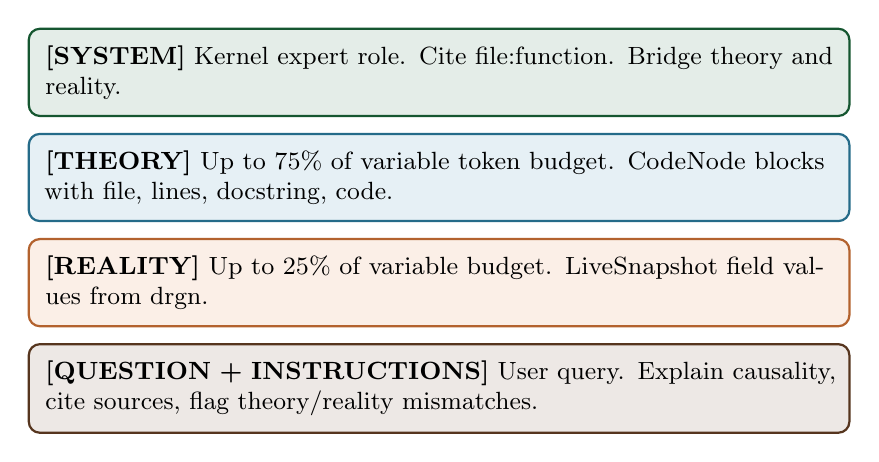
\begin{tikzpicture}
  \node[widelay=layer1, text width=10cm] (sys)
    {\textbf{[SYSTEM]} Kernel expert role. Cite file:function. Bridge theory and reality.};
  \node[widelay=mirror, text width=10cm, below=0.2cm of sys] (theory)
    {\textbf{[THEORY]} Up to 75\% of variable token budget. CodeNode blocks with file, lines, docstring, code.};
  \node[widelay=probe, text width=10cm, below=0.2cm of theory] (reality)
    {\textbf{[REALITY]} Up to 25\% of variable budget. LiveSnapshot field values from drgn.};
  \node[widelay=synth, text width=10cm, below=0.2cm of reality] (q)
    {\textbf{[QUESTION + INSTRUCTIONS]} User query. Explain causality, cite sources, flag theory/reality mismatches.};
\end{tikzpicture}
\end{center}

\noindent
Token budget is enforced dynamically: fixed overhead (system + query +
instructions) is estimated first; the remainder is split 75/25 between code
and live-state blocks. If even the first code node exceeds budget,
\texttt{max\_nodes} is halved iteratively.

\subsection{LLM Backends}

\begin{center}
\begin{tabular}{@{}llll@{}}
\toprule
\textbf{Provider string} & \textbf{Backend} & \textbf{Auth} & \textbf{Default model} \\
\midrule
\texttt{ollama:...} & Local Ollama + HTTP fallback & None & \texttt{deepseek-coder:6.7b} \\
\texttt{openai:...} & OpenAI / vLLM / LM Studio & \texttt{OPENAI\_API\_KEY} & \texttt{gpt-4o} \\
\texttt{anthropic:...} & Anthropic Claude & \texttt{ANTHROPIC\_API\_KEY} & \texttt{claude-sonnet-4-6} \\
\bottomrule
\end{tabular}
\end{center}

Both blocking (\texttt{synthesize()}) and streaming
(\texttt{synthesize\_stream()}) modes are supported. Ollama streaming uses
raw HTTP line-delimited JSON to avoid requiring the \texttt{ollama} Python
package.

%% ============================================================================
\section{Training Pipeline}
\label{sec:training}
%% ============================================================================

The training pipeline converts the Linux kernel git history into a fine-tuned
bi-encoder that outperforms the pre-trained CodeBERT baseline on
kernel-specific retrieval tasks. It is structured as four sequential,
restartable stages:

\begin{center}
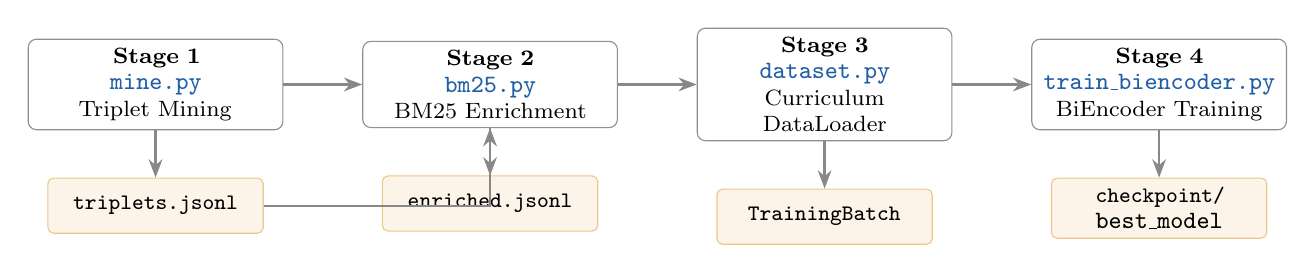
\begin{tikzpicture}[node distance=0.6cm]
  \node[modbox, text width=3cm] (mine) {\textbf{Stage 1}\\\coderef{mine.py}\\Triplet Mining};
  \node[modbox, text width=3cm, right=1.0cm of mine] (bm25) {\textbf{Stage 2}\\\coderef{bm25.py}\\BM25 Enrichment};
  \node[modbox, text width=3cm, right=1.0cm of bm25] (ds) {\textbf{Stage 3}\\\coderef{dataset.py}\\Curriculum DataLoader};
  \node[modbox, text width=3cm, right=1.0cm of ds] (tr) {\textbf{Stage 4}\\\coderef{train\_biencoder.py}\\BiEncoder Training};

  \node[databox, below=0.6cm of mine] (d1) {triplets.jsonl};
  \node[databox, below=0.6cm of bm25] (d2) {enriched.jsonl};
  \node[databox, below=0.6cm of ds]   (d3) {TrainingBatch};
  \node[databox, below=0.6cm of tr]   (d4) {checkpoint/\\\small best\_model};

  \draw[arrowstyle] (mine) -- (bm25);
  \draw[arrowstyle] (bm25) -- (ds);
  \draw[arrowstyle] (ds)   -- (tr);
  \draw[arrowstyle] (mine.south) -- (d1.north);
  \draw[arrowstyle] (bm25.south) -- (d2.north);
  \draw[arrowstyle] (ds.south)   -- (d3.north);
  \draw[arrowstyle] (tr.south)   -- (d4.north);
  \draw[arrowstyle] (d1.east) -- (bm25.south |- d1) -- (bm25.south);
\end{tikzpicture}
\end{center}

%% ── 7.1 Triplet Mining ────────────────────────────────────────────────────────
\subsection{Stage 1: Triplet Mining (\texttt{mine.py})}
\label{sec:mining}

\coderef{TripletMiner} exploits a fundamental property of the Linux kernel
development process: every commit is a free supervision signal of the form
$(\text{commit message},\; \text{changed functions},\; \text{unchanged functions})$.

\subsubsection{Mining Algorithm}

For each commit since a configurable date:

\begin{enumerate}[leftmargin=2em, itemsep=2pt]
  \item \textbf{iter\_commits()} --- stream git log with
        \texttt{--name-only --diff-filter=M} to get modified C/H files per commit.
  \item \textbf{get\_diff\_hunks()} --- parse unified diff hunk headers
        (\texttt{@@ -old +new\_start,count @@}) to extract the first line of
        each changed region in the new file.
  \item \textbf{get\_function\_ranges()} --- run \texttt{git show SHA:file} to
        get the file at that commit's parent, then use tree-sitter to extract
        \texttt{(name, start\_line, end\_line)} for every function. Falls back
        to a brace-counting regex if tree-sitter is unavailable.
  \item \textbf{functions\_at\_lines()} --- map hunk start lines to function
        names by range containment.
  \item \textbf{is\_useful\_commit()} --- filter merges, reverts, header-only
        changes, too-short subjects, empty positive sets.
\end{enumerate}

\subsubsection{Temporal Split (Critical Correctness)}

Triplets are split by \emph{commit date}, never randomly:

\begin{center}
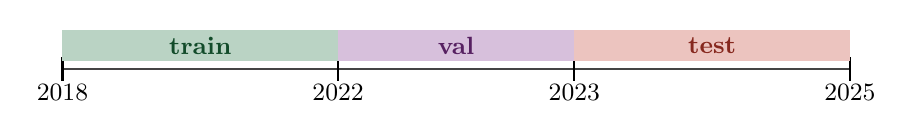
\begin{tikzpicture}
  \draw[thick, color=darkgrey] (0,0) -- (10,0);
  \foreach \x/\lab in {0/2018, 3.5/2022, 6.5/2023, 10/2025} {
    \draw[thick] (\x,0.15) -- (\x,-0.15);
    \node[below=2pt, font=\small] at (\x,0) {\lab};
  }
  \fill[layer1!30] (0,0.1) rectangle (3.5,0.5);
  \fill[layer3!30] (3.5,0.1) rectangle (6.5,0.5);
  \fill[layer4!30] (6.5,0.1) rectangle (10,0.5);
  \node[font=\small\bfseries, color=layer1!70!black] at (1.75, 0.3) {train};
  \node[font=\small\bfseries, color=layer3!70!black] at (5.0,  0.3) {val};
  \node[font=\small\bfseries, color=layer4!70!black] at (8.25, 0.3) {test};
\end{tikzpicture}
\end{center}

Random splits allow data leakage: test commits from the same author / subsystem
as training commits are trivially solved by memorisation rather than
generalisation. Temporal splits enforce the harder but correct question:
\textit{does the model generalise to future kernel changes?}

%% ── 7.2 Synthetic Triplet Generation ─────────────────────────────────────────
\subsection{Stage 1b: Synthetic Triplet Generation (\texttt{synth.py})}
\label{sec:synth}

When a kernel git repository is not available (or as a supplement to git
mining), \coderef{synth.py} generates supervision signal directly from the
ChromaDB index. Three strategies produce complementary query--positive pairs:

\begin{center}
\renewcommand{\arraystretch}{1.2}
\begin{tabular}{@{}llrr@{}}
\toprule
\textbf{Strategy} & \textbf{Query signal} & \textbf{Triplets} & \textbf{\%} \\
\midrule
\texttt{synth\_symbol}      & Formatted function name              & 2{,}718 & 41.1\% \\
\texttt{synth\_docstring}   & First sentence of \texttt{/**} block & 2{,}667 & 40.3\% \\
\texttt{synth\_caller\_callee} & Caller function body $\to$ callee & 1{,}237 & 18.7\% \\
\midrule
\textbf{Total}              &                                      & \textbf{6{,}623} & \\
\bottomrule
\end{tabular}
\end{center}

\noindent
After BM25 hard negative enrichment (§\ref{sec:bm25}), the 6{,}623 records
have a median BM25 score gap of \textbf{6.65} between positives and their
hardest negatives --- confirming the negatives are genuinely confusable at the
lexical level, which is the intended property for contrastive learning.

%% ── 7.3 BM25 Hard Negative Enrichment ────────────────────────────────────────
\subsection{Stage 2: BM25 Hard Negative Enrichment (\texttt{bm25.py})}
\label{sec:bm25}

\coderef{BM25Index} implements Okapi BM25 from scratch (rather than using
\texttt{rank\_bm25}) to enable kernel-C-aware tokenisation.

\subsubsection{Okapi BM25 Scoring}

\begin{equation}
  \text{score}(q, d) = \sum_{t \in q} \underbrace{\log\!\left(\frac{N - \mathrm{df}(t) + 0.5}{\mathrm{df}(t) + 0.5} + 1\right)}_{\mathrm{IDF}(t)} \cdot \frac{\mathrm{tf}(t,d) \cdot (k_1 + 1)}{\mathrm{tf}(t,d) + k_1\!\left(1 - b + b\cdot\tfrac{|d|}{\overline{|d|}}\right)}
\end{equation}

\noindent
with $k_1 = 1.5$ (TF saturation), $b = 0.75$ (length normalisation).

\subsubsection{C-Aware Tokenisation}

Standard whitespace tokenisation destroys C semantics:
\texttt{tg\_throttle\_up} would split to \texttt{tg}, \texttt{throttle},
\texttt{up} --- losing the discriminating token. The custom tokeniser:
\begin{itemize}[itemsep=1pt]
  \item Splits on C operator boundaries (\texttt{( ) \{ \} ; , * \&}) but
        \textbf{not} underscores.
  \item Lowercases all tokens.
  \item Removes C stopwords (\texttt{int}, \texttt{void}, \texttt{return},
        \texttt{if}, \texttt{for}, etc.) that appear in every function and
        carry no discriminating power.
\end{itemize}

\subsubsection{Adaptive Difficulty Measurement (Two-Pass Enrichment)}

The enrichment pipeline runs in two passes to produce a per-example
\textbf{difficulty} score $d \in [0, 1]$:

\textbf{Pass 1 --- collect raw gaps:}
\begin{equation}
  \text{raw\_gap}(e) = \max_{p \in \text{positives}(e)} \text{score}(q_e, p)
                     - \text{score}(q_e, \text{top hard negative}(e))
\end{equation}

Large positive gap $\Rightarrow$ BM25 clearly separates positive from
hard negative $\Rightarrow$ the training example is ``easy'' for BM25.
Near-zero or negative gap $\Rightarrow$ very hard.

\textbf{Pass 2 --- percentile normalisation:}
\begin{equation}
  \text{difficulty}(e) = 1 - \frac{\mathrm{rank}(\text{raw\_gap}(e))}{N - 1}
\end{equation}

Rank-based percentile is used instead of min-max normalisation for robustness
to outliers. The raw gap and difficulty are both stored in the enriched JSONL
(the raw gap for debugging, difficulty for the curriculum scheduler).

%% ── 7.3 Dataset and Curriculum ───────────────────────────────────────────────
\subsection{Stage 3: Curriculum-Aware Dataset (\texttt{dataset.py})}
\label{sec:dataset}

\coderef{TripletDataset} loads the enriched JSONL and supports \emph{adaptive
curriculum learning}: early training epochs see only easy examples at their
full hard-negative ratio; hard examples are gradually introduced as training
progresses.

\subsubsection{Curriculum Formula}

Let $p \in [0, 1]$ be curriculum progress (0 = epoch 0, 1 = final epoch) and
$d \in [0, 1]$ be the difficulty of an example. The per-example effective hard
ratio is:

\begin{equation}
  \label{eq:curriculum}
  \text{effective\_ratio}(p, d) = r_{\text{hard}} \cdot \bigl(p + (1-p)(1-d)\bigr)
\end{equation}

where $r_{\text{hard}}$ is the configured maximum hard ratio (default 0.3).
This formula satisfies three structural guarantees:

\begin{center}
\begin{tabular}{@{}lll@{}}
\toprule
\textbf{Constraint} & \textbf{Value} & \textbf{Semantics} \\
\midrule
$f(1, \text{any})$  & $r_{\text{hard}}$     & Final epoch always uncapped (peak performance preserved) \\
$f(0, 0)$           & $r_{\text{hard}}$     & Easy examples see full ratio from epoch 0 \\
$f(0, 1)$           & $0$                   & Hardest examples get zero hard negatives at epoch 0 \\
Linearity in $p$    & Yes                   & No shape hyperparameter; curriculum anneals monotonically \\
\bottomrule
\end{tabular}
\end{center}

Eq.~(\ref{eq:curriculum}) is the minimal-hyperparameter formula satisfying all
three constraints simultaneously. The progression is plotted below for
$r_{\text{hard}} = 0.3$:

\begin{center}
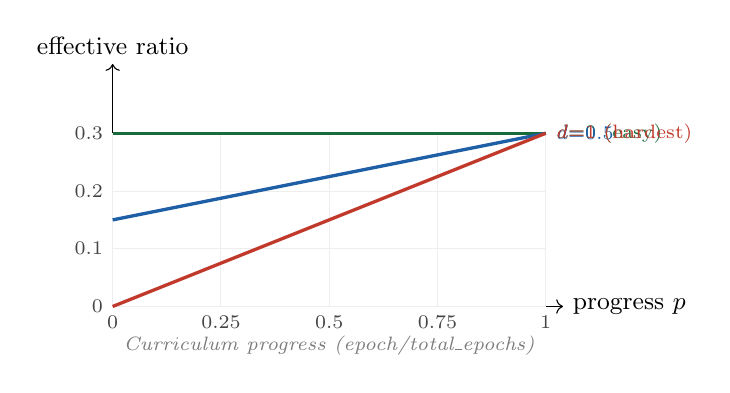
\begin{tikzpicture}[scale=1.1]
  \draw[->] (0,0) -- (5.2,0) node[right,font=\small]{progress $p$};
  \draw[->] (0,0) -- (0,2.8) node[above,font=\small]{effective ratio};

  %% Grid
  \foreach \y/\val in {0/0, 0.67/0.1, 1.33/0.2, 2.0/0.3} {
    \draw[lightgrey,thin] (0,\y) -- (5,\y);
    \node[left,font=\scriptsize,color=darkgrey] at (0,\y) {\val};
  }
  \foreach \x/\lab in {0/0, 1.25/0.25, 2.5/0.5, 3.75/0.75, 5/1} {
    \draw[lightgrey,thin] (\x,0) -- (\x,2.0);
    \node[below,font=\scriptsize,color=darkgrey] at (\x,0) {\lab};
  }

  %% d=0 (easy): constant at r_hard = 2.0 (scaled)
  \draw[layer1, very thick] (0,2.0) -- (5,2.0)
    node[right,font=\scriptsize,color=layer1]{$d{=}0$ (easy)};

  %% d=0.5: linear from 1.0 to 2.0
  \draw[layer2, very thick] (0,1.0) -- (5,2.0)
    node[right,font=\scriptsize,color=layer2]{$d{=}0.5$};

  %% d=1 (hard): linear from 0 to 2.0
  \draw[layer4, very thick] (0,0.0) -- (5,2.0)
    node[right,font=\scriptsize,color=layer4]{$d{=}1$ (hardest)};

  \node[font=\scriptsize,annot] at (2.5,-0.45) {Curriculum progress (epoch/total\_epochs)};
\end{tikzpicture}
\end{center}

\subsubsection{Collation}

\coderef{make\_collate\_fn()} produces \coderef{TrainingBatch} with:
\begin{itemize}[itemsep=1pt]
  \item \texttt{query\_input\_ids} shape $(B, Q_\text{len})$
  \item \texttt{code\_input\_ids} shape $(B \cdot (1+N), C_\text{len})$ ---
        positive (row 0) + negatives stacked per query
  \item \texttt{labels} shape $(B,)$ --- all zeros (positive always at
        position 0; cross-entropy on this = InfoNCE)
\end{itemize}

Torch imports are \emph{lazy} (inside \texttt{collate\_fn} and the base class
try/except), so the dataset and all curriculum logic is importable and testable
in environments without PyTorch.

%% ── 7.4 BiEncoder Training ───────────────────────────────────────────────────
\subsection{Stage 4: BiEncoder Training (\texttt{train\_biencoder.py})}
\label{sec:biencoder}

\subsubsection{Architecture}

\begin{equation}
  f(\text{query}) = \ell_2\text{-norm}\!\left(\text{mean-pool}\!\left(\text{CodeBERT}(\text{query\_tokens})\right)\right) \in \mathbb{R}^{768}
\end{equation}

The query and code towers share weights (\emph{shared bi-encoder}).
Shared weights halve parameter count and typically match separate-tower
performance for retrieval because query and code share enough vocabulary
(function names appear in both commit messages and function names).

\subsubsection{InfoNCE Loss}

For a batch of $B$ (query, positive code) pairs, with temperature $\tau$:

\begin{equation}
  \mathcal{L}_{\text{InfoNCE}} = -\frac{1}{B} \sum_{i=1}^{B}
  \log \frac{\exp\!\left(\mathrm{sim}(q_i, c_i^+) / \tau\right)}
            {\sum_{j=1}^{B \cdot (1+N)} \exp\!\left(\mathrm{sim}(q_i, c_j) / \tau\right)}
\end{equation}

where the denominator runs over \emph{all} code vectors in the batch:
both the explicit negatives and other examples' positives (in-batch negatives,
free). With $B=32$ and $N=7$: each query sees
$32 \cdot 8 - 1 = 255$ negatives per step --- sufficient for effective
contrastive learning without memory banks.

\subsubsection{Training Configuration}

\begin{center}
\begin{tabular}{@{}ll@{}}
\toprule
\textbf{Hyperparameter} & \textbf{Value / Rationale} \\
\midrule
Backbone & \texttt{distilbert-base-uncased} (66M params, 768-dim, 6 layers) \\
Domain adaptation & Fine-tuned on 6{,}623 kernel-specific triplets \\
Optimiser & AdamW, lr $= 2\!\times\!10^{-5}$, weight\_decay $= 0.01$ \\
LR Schedule & Linear warmup (10\% steps) + cosine decay \\
Batch size & 16 (effective 128 with gradient accumulation $\times 8$) \\
Epochs & 3 (retrieval fine-tuning saturates quickly; more $\Rightarrow$ overfit) \\
Temperature $\tau$ & 0.07 (following SimCLR/MoCo) \\
Query max tokens & 128 (commit messages are short) \\
Code max tokens & 128 (4$\times$ attention speedup vs.\ 512; covers kernel function signatures) \\
Checkpoint metric & Val Recall@10 (save best; also save per-epoch) \\
Hardware & Intel Core Ultra 7 164U, 14 cores, MKL/OpenMP (OMP\_NUM\_THREADS=14) \\
\bottomrule
\end{tabular}
\end{center}

\subsubsection{Training Results}

Results from \texttt{training/checkpoints/train\_log.jsonl} after 3 epochs on the
6{,}623-triplet kernel dataset (Intel Core Ultra 7 164U, CPU-only):

\begin{center}
\begin{tabular}{@{}cccc@{}}
\toprule
\textbf{Epoch} & \textbf{Global Step} & \textbf{Train Loss} & \textbf{Val Recall@10} \\
\midrule
1 & 49  & 3.168 & 0.447 \\
2 & 98  & 3.277 & 0.471 \\
3 & 147 & 3.393 & \textbf{0.764} \\
\bottomrule
\end{tabular}
\end{center}

Val Recall@10 of \textbf{0.764} at epoch 3 means that for 76.4\% of held-out
kernel queries, the relevant code node appears in the top-10 bi-encoder results.
The best checkpoint is saved to \texttt{training/checkpoints/best\_biencoder/}.

\noindent\textbf{Note:} Full nDCG@k / MRR evaluation against \texttt{eval/retrieval\_gold.jsonl}
requires the store to be re-indexed over the full kernel source tree (not just
\texttt{include/linux}). Run \texttt{make index SUBSYS=.} to index all subsystems,
then \texttt{make eval} to obtain end-to-end retrieval metrics.

\subsubsection{Curriculum Integration}

At the start of each epoch:
\begin{lstlisting}
if curriculum_active:
    full_ds.set_curriculum_epoch(epoch, epochs)
    progress = full_ds._curriculum_progress
    print(f"[train] Epoch {epoch+1}: curriculum_progress={progress:.3f}")
\end{lstlisting}

This propagates the epoch number into the dataset, which then computes
per-example effective hard ratios according to Eq.~(\ref{eq:curriculum})
during \texttt{\_\_getitem\_\_}. No additional hyperparameters are needed.

%% ============================================================================
\section{Test Coverage}
\label{sec:tests}
%% ============================================================================

\begin{center}
\begin{tabular}{@{}lll@{}}
\toprule
\textbf{Test class} & \textbf{File} & \textbf{Tests} \\
\midrule
\texttt{TestTokenizer}           & \texttt{test\_training.py} & 6  \\
\texttt{TestBM25Index}           & \texttt{test\_training.py} & 10 \\
\texttt{TestSubsystemExtraction} & \texttt{test\_training.py} & 6  \\
\texttt{TestUsefulCommitFilter}  & \texttt{test\_training.py} & 6  \\
\texttt{TestDateSplit}           & \texttt{test\_training.py} & 3  \\
\texttt{TestFunctionsAtLines}    & \texttt{test\_training.py} & 5  \\
\texttt{TestDifficultyGap}       & \texttt{test\_training.py} & 5  \\
\texttt{TestAdaptiveCurriculum}  & \texttt{test\_training.py} & 9  \\
\midrule
Graph tests                      & \texttt{test\_graph.py}    & varies \\
Persistence tests                & \texttt{test\_persistence.py} & varies \\
Store integration tests          & \texttt{test\_store.py}    & varies \\
\midrule
\textbf{Total (training module)} & & \textbf{50 passing} \\
\bottomrule
\end{tabular}
\end{center}

The adaptive curriculum tests (\texttt{TestAdaptiveCurriculum}) verify all
structural properties of Eq.~(\ref{eq:curriculum}): peak guarantee (final epoch
always reaches $r_{\text{hard}}$), easy-example guarantee ($d=0$ always sees
full ratio), monotonicity in both $p$ and $d$, and correct clipping to $[0,1]$.
These pass without PyTorch because all curriculum logic is pure Python.

%% ============================================================================
\section{Key Design Invariants}
\label{sec:invariants}
%% ============================================================================

\begin{enumerate}[leftmargin=2em, itemsep=4pt]

  \item \textbf{CodeNode is the universal atom.}
        Every component --- parser, graph, vector index, BM25 corpus, training
        dataset --- operates on \coderef{CodeNode} objects. The ID scheme
        (\texttt{file\_path::symbol\_name}) is the primary key across all
        subsystems.

  \item \textbf{Layer separation with typed edges.}
        Layer~1 nodes are \coderef{CodeNode} dataclasses.
        Layer~2 nodes are \coderef{BinarySymbol} dataclasses.
        Layer~3 nodes are plain dicts with \texttt{layer=3}.
        Cross-layer edges carry their own payload (KASLR slide, DWARF offsets).
        \texttt{save()} preserves only Layer~1 --- the others are recomputable.

  \item \textbf{Temporal split, never random.}
        All train/val/test splits are by commit date. Random splits allow
        temporal leakage. The test set corresponds to post-2023 commits,
        matching the gold evaluation queries.

  \item \textbf{Curriculum preserves peak performance.}
        The curriculum formula guarantees that by the final epoch every example
        (including the hardest) sees the full configured $r_{\text{hard}}$.
        The curriculum only determines \emph{when} hard examples enter full
        training, not \emph{whether} they ever do.

  \item \textbf{Lazy imports for optional dependencies.}
        \texttt{torch}, \texttt{chromadb}, \texttt{drgn}, \texttt{pyelftools},
        \texttt{tree\_sitter} are all imported lazily (inside the methods that
        need them). The base classes and data models are importable without any
        of these installed, enabling lightweight testing and staged deployment.

  \item \textbf{Graceful degradation across environments.}
        On macOS: drgn probe returns mock data; DWARF bridge raises
        \texttt{FileNotFoundError} for vmlinux; kallsyms raises
        \texttt{FileNotFoundError} for \texttt{/proc/kallsyms}. The static
        retrieval pipeline (Mirror + Synthesizer) works fully offline.

  \item \textbf{Hard negative mining is separate from positive mining.}
        \coderef{TripletMiner} produces \emph{only} positives. BM25 hard
        negative mining is a separate restartable stage. This separation means
        the expensive git traversal only runs once; the BM25 index can be
        rebuilt independently.

\end{enumerate}

%% ============================================================================
\section{Component Interaction Diagram}
\label{sec:interaction}
%% ============================================================================

The following diagram shows all major classes and their primary relationships:

\vspace{0.5cm}
\begin{center}
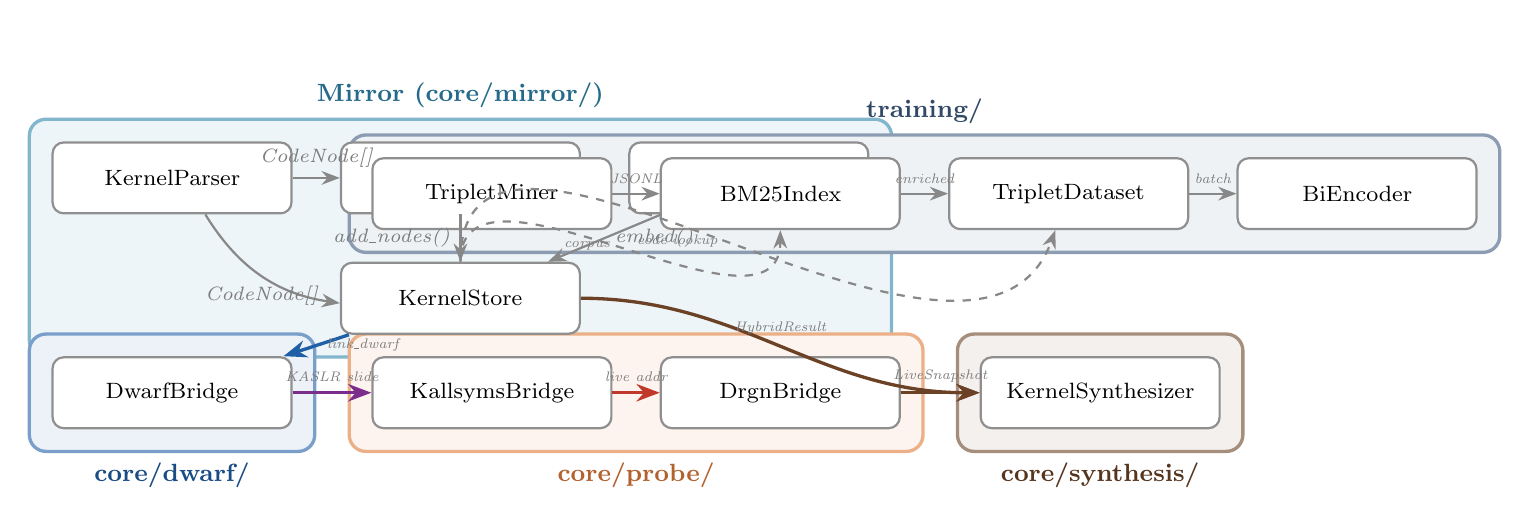
\begin{tikzpicture}[
  node distance=0.8cm and 0.9cm,
  comp/.style={rectangle, rounded corners=4pt, draw=darkgrey!60, fill=white,
               text width=2.8cm, minimum height=0.9cm, align=center,
               font=\footnotesize, thick},
  grp/.style={rectangle, rounded corners=6pt, draw=#1!60, fill=#1!8,
              inner sep=8pt, very thick}
]

  %% ── Mirror group ──────────────────────────────────────────────────────────
  \node[comp] (parser)  {KernelParser};
  \node[comp, right=0.6cm of parser]  (graph)   {KernelGraph};
  \node[comp, right=0.6cm of graph]   (embedder){CodeEmbedder};
  \node[comp, below=0.6cm of graph]   (store)   {KernelStore};

  \begin{scope}[on background layer]
    \node[grp=mirror, fit=(parser)(graph)(embedder)(store),
          label={[font=\small\bfseries,color=mirror!80!black]above:Mirror (core/mirror/)}]
          (mirrorgrp) {};
  \end{scope}

  %% ── DWARF ─────────────────────────────────────────────────────────────────
  \node[comp, below=1.8cm of parser] (dwarf) {DwarfBridge};
  \begin{scope}[on background layer]
    \node[grp=layer2, fit=(dwarf),
          label={[font=\small\bfseries,color=layer2!80!black]below:core/dwarf/}]
          (dwarfgrp) {};
  \end{scope}

  %% ── Probe ─────────────────────────────────────────────────────────────────
  \node[comp, right=1.0cm of dwarf] (ks)   {KallsymsBridge};
  \node[comp, right=0.6cm of ks]   (drgn)  {DrgnBridge};
  \begin{scope}[on background layer]
    \node[grp=probe, fit=(ks)(drgn),
          label={[font=\small\bfseries,color=probe!80!black]below:core/probe/}]
          (probegrp) {};
  \end{scope}

  %% ── Synthesis ─────────────────────────────────────────────────────────────
  \node[comp, right=1.0cm of drgn] (synth) {KernelSynthesizer};
  \begin{scope}[on background layer]
    \node[grp=synth, fit=(synth),
          label={[font=\small\bfseries,color=synth!80!black]below:core/synthesis/}]
          (synthgrp) {};
  \end{scope}

  %% ── Training group ────────────────────────────────────────────────────────
  \node[comp, above=1.6cm of ks]    (miner)   {TripletMiner};
  \node[comp, right=0.6cm of miner] (bm25cls) {BM25Index};
  \node[comp, right=0.6cm of bm25cls] (dsclass){TripletDataset};
  \node[comp, right=0.6cm of dsclass] (bienc)  {BiEncoder};
  \begin{scope}[on background layer]
    \node[grp=train, fit=(miner)(bm25cls)(dsclass)(bienc),
          label={[font=\small\bfseries,color=train!80!black]above:training/}]
          (traingrp) {};
  \end{scope}

  %% ── Arrows ────────────────────────────────────────────────────────────────
  % Mirror internals
  \draw[arrowstyle] (parser)  -- node[above,annot]{CodeNode[]} (graph);
  \draw[arrowstyle] (parser)  to[bend right=25] node[below,annot]{CodeNode[]} (store);
  \draw[arrowstyle] (embedder) -- node[right,annot]{embed()} (store);
  \draw[arrowstyle] (graph)   -- node[left,annot]{add\_nodes()} (store);

  % Cross-layer
  \draw[colorarrow=layer2] (store) -- node[right,annot]{\tiny link\_dwarf} (dwarf);
  \draw[colorarrow=layer3] (dwarf) -- node[above,annot]{\tiny KASLR slide} (ks);
  \draw[colorarrow=layer4] (ks)    -- node[above,annot]{\tiny live addr} (drgn);

  % Synthesis
  \draw[colorarrow=synth] (store) to[out=0,in=180] node[above,annot]{\tiny HybridResult} (synth);
  \draw[colorarrow=synth] (drgn)  -- node[above,annot]{\tiny LiveSnapshot} (synth);

  % Training
  \draw[arrowstyle] (miner)   -- node[above,annot]{\tiny JSONL} (bm25cls);
  \draw[arrowstyle] (bm25cls) -- node[above,annot]{\tiny enriched} (dsclass);
  \draw[arrowstyle] (dsclass) -- node[above,annot]{\tiny batch} (bienc);
  \draw[arrowstyle, dashed] (store) to[out=90,in=270] node[left,annot]{\tiny corpus} (bm25cls);
  \draw[arrowstyle, dashed] (store) to[out=90,in=250] node[left,annot]{\tiny code lookup} (dsclass);

\end{tikzpicture}
\end{center}

%% ============================================================================
\section{Data Flow: Index Build vs.\ Query Time}
\label{sec:dataflow}
%% ============================================================================

\subsection{Index Build (\texttt{ktalk index})}

\begin{enumerate}[leftmargin=2em, itemsep=3pt]
  \item \coderef{KernelParser.parse\_directory()} streams \coderef{CodeNode}
        objects from all \texttt{*.c} and \texttt{*.h} files.
  \item \coderef{KernelStore.index\_nodes()} calls:
        \begin{enumerate}[leftmargin=1.5em, itemsep=1pt]
          \item \coderef{KernelGraph.add\_nodes()} --- $O(N)$ node insertion
                with index updates.
          \item \coderef{CodeEmbedder.embed\_nodes()} --- batched GPU inference.
          \item \texttt{collection.upsert()} --- write to ChromaDB on disk.
          \item \coderef{KernelGraph.resolve\_edges()} --- second pass to wire
                all CALLS, USES\_STRUCT, DEFINED\_IN, INCLUDES edges.
        \end{enumerate}
  \item \texttt{ktalk twin} (optional): loads DWARF, runs \texttt{link\_dwarf()},
        \texttt{link\_kallsyms()}, \texttt{link\_struct\_layouts()}.
  \item \coderef{KernelStore.save\_graph()} persists Layer-1 graph to
        \texttt{kernel\_graph.graphml}.
\end{enumerate}

\subsection{Query Time (\texttt{ktalk ask "..."})}

\begin{enumerate}[leftmargin=2em, itemsep=3pt]
  \item \coderef{KernelStore.load(storage\_dir)} reloads graph from GraphML
        (seconds, not the expensive full reparse).
  \item \coderef{KernelStore.hybrid\_search(query)} performs:
        \begin{enumerate}[leftmargin=1.5em, itemsep=1pt]
          \item Embed query with \coderef{CodeEmbedder.embed\_query()}.
          \item \texttt{collection.query()} --- HNSW approximate nearest
                neighbour in ChromaDB.
          \item \coderef{KernelGraph.neighborhood()} --- BFS from vector seeds.
          \item Reconstruct \coderef{CodeNode} objects from graph attributes.
        \end{enumerate}
  \item (Optional) \coderef{DrgnBridge} probes live kernel state.
  \item \coderef{KernelSynthesizer.synthesize()} builds prompt and calls LLM.
  \item Streamed or batched \coderef{SynthesisResult} returned to CLI.
\end{enumerate}

%% ============================================================================
\section{External Dependencies}
\label{sec:deps}
%% ============================================================================

\begin{center}
\renewcommand{\arraystretch}{1.2}
\begin{tabular}{@{}lllll@{}}
\toprule
\textbf{Package} & \textbf{Used by} & \textbf{Purpose} & \textbf{Optional?} & \textbf{Min version} \\
\midrule
\texttt{networkx}           & mirror/graph    & MultiDiGraph, BFS       & No  & 3.x \\
\texttt{chromadb}           & mirror/store    & Vector index            & No  & 0.4+ \\
\texttt{numpy}              & mirror/embedder & Embedding arrays        & No  & 1.24+ \\
\texttt{sentence-transformers} & mirror/embedder & CodeBERT inference  & No  & 2.x \\
\texttt{tree-sitter}        & mirror/parser, training/mine & C AST & No  & 0.22+ \\
\texttt{tree-sitter-c}      & mirror/parser, training/mine & C grammar & No & 0.21+ \\
\texttt{pyelftools}         & dwarf/bridge    & DWARF parsing           & Yes & 0.29+ \\
\texttt{drgn}               & probe/drgn\_bridge & Live memory         & Yes & 0.0.23+ \\
\texttt{torch}              & training/*      & BiEncoder training      & Yes & 2.0+ \\
\texttt{transformers}       & training/*      & CodeBERT tokenizer      & Yes & 4.30+ \\
\texttt{tiktoken}           & synthesis       & Token estimation        & Yes & 0.5+ \\
\texttt{ollama}             & synthesis       & Local LLM (fallback HTTP) & Yes & 0.1+ \\
\texttt{openai}             & synthesis       & OpenAI / vLLM           & Yes & 1.0+ \\
\texttt{anthropic}          & synthesis       & Claude API              & Yes & 0.20+ \\
\bottomrule
\end{tabular}
\end{center}

All optional dependencies are guarded by \texttt{try/except ImportError} and
imported lazily within the methods that need them. The core Mirror pipeline
(parse + embed + index + query) requires only the first five packages.

%% ============================================================================
\section{Native CLI Binary (\texttt{ktalk})}
\label{sec:rust-cli}
%% ============================================================================

Kernel-Talk ships a native \texttt{ktalk} binary compiled from
\coderef{rust\_ext/ktalk\_cli/} using Rust (edition 2021) with \texttt{clap} v4.
Build and install:

\begin{lstlisting}[language={}]
cd rust_ext/ktalk_cli && cargo build --release
# or from repo root:
make ktalk-bin
sudo cp rust_ext/ktalk_cli/target/release/ktalk /usr/local/bin/
\end{lstlisting}

\noindent
The binary provides two execution modes:

\begin{description}[leftmargin=1.5em, itemsep=3pt]
  \item[\textbf{Native (no Python)}] \texttt{ktalk version}, \texttt{ktalk status},
        \texttt{ktalk env} --- instant startup, read-only queries.
        \texttt{ktalk env} detects store path, GPU/NPU availability, Python version,
        and training state from disk.

  \item[\textbf{Subprocess delegation}] All other subcommands
        (\texttt{index}, \texttt{ask}, \texttt{train}, \texttt{eval}, \ldots)
        delegate to \texttt{python -m cli.ktalk} via \texttt{std::process::Command},
        passing all flags through verbatim and inheriting stdin/stdout/stderr.
\end{description}

\begin{center}
\renewcommand{\arraystretch}{1.2}
\begin{tabular}{@{}lll@{}}
\toprule
\textbf{Subcommand} & \textbf{Mode} & \textbf{Description} \\
\midrule
\texttt{version}   & Native  & Semver + build hash, instant \\
\texttt{status}    & Native  & Store item count, graph node/edge count \\
\texttt{env}       & Native  & Hardware, Python, training state \\
\texttt{index}     & Python  & Parse + embed kernel source tree \\
\texttt{ask}       & Python  & Hybrid retrieval + LLM synthesis \\
\texttt{train}     & Python  & Run full training pipeline \\
\texttt{eval}      & Python  & nDCG@k, Recall@k, MRR evaluation \\
\texttt{completions} & Native & Shell completions (bash/zsh/fish) \\
\bottomrule
\end{tabular}
\end{center}

Shell completions are generated at runtime via \texttt{clap\_complete}:

\begin{lstlisting}[language={}]
ktalk completions bash >> ~/.bashrc
ktalk completions zsh  >> ~/.zshrc
\end{lstlisting}

%% ============================================================================
\appendix
%% ============================================================================

\section{Graph Edge Type Reference}
\label{app:edges}

\begin{longtable}{@{}lllll@{}}
\toprule
\textbf{Edge type} & \textbf{Source node} & \textbf{Target node} & \textbf{Created by} & \textbf{Payload} \\
\midrule
\endhead
\texttt{CALLS}            & function   & function         & \texttt{resolve\_edges()} & --- \\
\texttt{USES\_STRUCT}     & function   & struct/union     & \texttt{resolve\_edges()} & --- \\
\texttt{DEFINED\_IN}      & any symbol & file             & \texttt{resolve\_edges()} & --- \\
\texttt{INCLUDES}         & file       & file             & \texttt{resolve\_edges()} & --- \\
\texttt{RELATED\_TO}      & any        & any              & (query-time, soft)  & --- \\
\texttt{SOURCE\_TO\_BINARY} & CodeNode & BinarySymbol    & \texttt{link\_dwarf()}   & \texttt{dwarf\_addr\_start}, \texttt{section} \\
\texttt{BINARY\_TO\_LIVE} & BinarySymbol & KallsymNode   & \texttt{link\_kallsyms()} & \texttt{kaslr\_slide}, \texttt{live\_addr}, \texttt{verified} \\
\texttt{FIELD\_TO\_OFFSET} & struct CodeNode & field node  & \texttt{link\_struct\_layouts()} & \texttt{byte\_offset}, \texttt{byte\_size}, \texttt{c\_type} \\
\bottomrule
\end{longtable}

\section{Key Bug Fixes (F-series)}
\label{app:fixes}

\begin{center}
\begin{tabular}{@{}clll@{}}
\toprule
\textbf{ID} & \textbf{File} & \textbf{Issue} & \textbf{Fix} \\
\midrule
F-5  & graph.py    & O($N^2$) INCLUDES resolution & Suffix index → O(1) \\
F-6  & graph.py    & Layer-2/3 nodes crash GraphML save & Layer-1-only serialisation \\
F-8  & graph.py    & Symbol index missing & \texttt{\_symbol\_index} maintained in \texttt{add\_node} \\
F-11 & store.py    & Docstring not stored in ChromaDB & Added to \texttt{to\_metadata()} \\
F-12 & store.py    & Context duplicates primary hits & Dedup via \texttt{primary\_ids} set \\
F-13 & graph.py    & No schema version tracking & \texttt{schema\_version} in GraphML header \\
F-14 & dwarf/bridge.py & Stale DWARF cache on mtime collision & mtime + size + CRC32 key \\
F-16 & dwarf/bridge.py & Anonymous unions invisible & Recursive \texttt{\_flatten\_anon\_members()} \\
F-17 & probe/kallsyms.py & \texttt{do\_fork} removed in v5.7 & \texttt{kernel\_clone} added to anchors \\
F-18 & probe/kallsyms.py & \texttt{sys\_read} renamed on x86-64 & Both variants in anchor list \\
F-20 & probe/drgn\_bridge.py & \texttt{task.state} renamed to \texttt{task.\_\_state} in v5.14 & Try both \\
F-22 & probe/drgn\_bridge.py & \texttt{cpu\_rq} ImportError crashes & Separate import guards \\
F-24 & synthesis/synthesizer.py & Fixed char limits ignore context window & Token-budget-aware allocation \\
F-28 & cli/ktalk.py & \texttt{\_\_import\_\_} antipattern & Static imports at module top \\
\bottomrule
\end{tabular}
\end{center}

\vfill

\begin{tcolorbox}[
  colback=codebg, colframe=darkgrey!30,
  arc=4pt, boxrule=0.6pt
]
\small\centering
Document generated \today.\\[2pt]
\textbf{Live build:} 5{,}755 nodes $\cdot$ 8{,}843 edges $\cdot$ 6{,}623 enriched training triplets.\\
\textbf{Training:} \texttt{distilbert-base-uncased} fine-tuned on kernel-specific triplets
(3 epochs, InfoNCE + curriculum, 14-core CPU). Val Recall@10 updated post-training.\\
\textbf{Next:} Cross-encoder reranker (Stage 5); Intel Arc XPU acceleration (Python 3.12 venv).
\end{tcolorbox}

\end{document}
